\documentclass[10pt]{article}
\usepackage[margin=0.75in]{geometry}
\usepackage{amsmath,amssymb,bm}
\usepackage{booktabs}
\usepackage{graphicx}
\usepackage{enumitem}
\usepackage[hidelinks]{hyperref}
\usepackage{caption}
\usepackage{titlesec}
\titlespacing*{\section}{0pt}{7pt}{3pt}
\titlespacing*{\paragraph}{0pt}{4pt}{1em}
\renewcommand{\topfraction}{0.9}\renewcommand{\textfraction}{0.07}\renewcommand{\floatpagefraction}{0.8}
\captionsetup{font=small,labelfont=bf,skip=4pt}
\setlist{itemsep=2pt,topsep=3pt,leftmargin=1.4em}
\setlength{\parskip}{2pt}
\linespread{1.0}
\setlength{\abovedisplayskip}{5pt}\setlength{\belowdisplayskip}{5pt}
\newcommand{\Tr}{\mathrm{Tr}}
\newcommand{\bPsi}{\bar\Psi}
\newcommand{\bQ}{\bar Q}
\newcommand{\rank}{\mathrm{rank}\,}
\title{\vspace{-1.6cm}\Large\textbf{Why Matrix SYK Models Do Not Have R-Charge Concentration}\vspace{-4pt}}
\author{}
\date{}

\begin{document}
\maketitle
\vspace{-1.1cm}
\begin{center}\begin{minipage}{0.97\textwidth}\small
\textbf{Abstract.} R-charge concentration --- all BPS states of an irreducible complex sitting in a single R-charge --- is the proposed fingerprint of a fortuitous, black-hole-like BPS sector, and Chen has conjectured that purely fermionic $U(N)$ matrix quantum mechanics with a cubic supercharge and three flavours realises it. We compute the BPS cohomology of these models exactly. The $U(N)$ weight decomposition splits the $Q$-complex into pieces of dimension $\le 10^4$ in place of $2^{pN^2}$, which puts $N\le5$ within reach of exact integer linear algebra; Kostant inversion converts weight-space cohomology into per-irrep BPS counts. The results are uniformly negative and follow a simple law. The BPS states occupy a window of \emph{consecutive} R-charges whose width grows linearly with the gauge rank: $W=N+1$ for $p=1,3$, $W=2N+1$ for $p=2,4$, $W=3N+1$ for $p=5$, with period four in $p$. Since the complexes are graded by $N_\Psi$ mod $q$ with $q=3$ fixed, a window of width $W>q$ cannot fit one degree per class, and concentration fails for every $N\ge3$. We then solve the problem analytically: at the maximal weight the complex factorises over the $\rank G$ Cartan directions into $\big(\Lambda^\bullet\mathbb C^p,\ \omega\wedge\big)^{\otimes \rank G}$, giving $W=\rank G\,(w_s-1)+1$ in closed form, and an Euler-characteristic argument forces $w_s\ge2$. Concentration therefore requires $\rank G\le q-1$, and solving for $w_s$ sharpens this to $\rank G\le2$ --- exactly $u(2)$ and $su(3)$. Chen's supporting $N=2$ evidence is one of the only two cases in the entire family where concentration holds, and it holds for kinematic reasons.
\end{minipage}\end{center}
\vspace{10pt}

\section{Introduction}

\paragraph{The models.}
The degrees of freedom are complex fermionic $N\times N$ matrices $\Psi^a_{ij}$, $a=1,\dots,p$, with $\{\Psi^a_{ij},\bPsi^b_{kl}\}=\delta^{ab}\delta_{il}\delta_{jk}$ and $U(N)$ acting by conjugation. All dynamics comes from a nilpotent supercharge,
\begin{equation}
Q=\sum_{a_1\dots a_q}C_{a_1\dots a_q}\Tr\!\big[\Psi^{a_1}\!\cdots\Psi^{a_q}\big],\qquad H=\{Q,\bQ\}\ge0,\qquad [N_\Psi,Q]=qQ ,
\label{eq:Q}
\end{equation}
with $N_\Psi=\Tr\Psi^a\bPsi^a$ the R-charge. Only odd $q$ is admissible: $\Tr[\Psi^q]$ picks up $(-1)^{q-1}$ under a cyclic shift, so it vanishes identically for even $q$, and $Q^2=0$ holds automatically precisely when $q$ is odd, because exchanging the two $q$-tuples in $C\otimes C$ is a permutation of $2q$ fermions with $q^2$ transpositions, contracted against a totally antisymmetric product. The case $q=3$, $p=1$ is Chen's exactly solvable single-matrix model~\cite{Chen:2025fortuity}, where $H$ is a function of the gauge Casimir; $q=3$, $p=3$ with Chen's couplings is the proposed ``matrix SYK'' model, for which the Casimir structure is lost.

BPS states are $E=0$ states, equivalently classes in $\ker Q/\operatorname{im}Q$. Because $Q$ is a gauge singlet and raises $N_\Psi$ by $q$, the cohomology splits into irreducible complexes labelled by the $U(N)$ irrep $\lambda$, the $\mathbb Z_p$ flavour charge $\omega$, and the residue $c=N_\Psi \bmod q$.

\paragraph{Concentration, and what is at stake.}
Chang, Chen, Sia and Yang~\cite{Chang:2024fortuitySYK} propose \emph{R-charge concentration} as the signature of a fortuitous BPS sector: along each irreducible complex with macroscopic index, all BPS states occupy a \emph{single} degree. In $\mathcal N=2$ SYK this holds, the BPS counts follow the $\cos(\pi k/3)$ profile of the $\mathcal N=2$ super-Schwarzian~\cite{Turiaci:2023N2JT,Fu:2016SUSYSYK}, and the index counts the BPS states exactly. Chen observes that his single-matrix model fails the test --- its BPS states span $N+1$ consecutive charges~\cite[(2.22)]{Chen:2025fortuity} --- and conjectures that with three flavours ``the magic number might be three'', citing an unpublished $N=2$ simulation that ``suggests'' concentration. Whether this survives $N\ge3$ has been open, and it is the question we settle.

\paragraph{Summary of results.}
\begin{itemize}
\item The BPS window is a run of consecutive R-charges centred on half filling, of width $W$ growing linearly in $N$: $W=N+1$ ($p=1,3$), $2N+1$ ($p=2,4$), $3N+1$ ($p=5$), with period four in $p$ (Table~\ref{tab:widths}). Exact counts at $N=2,3,4,5$ (Table~\ref{tab:profiles}).
\item Since the grading period is $q=3$, $W>3$ makes one-degree-per-class impossible. Concentration holds at $N=2$ and fails for every $N\ge3$ --- by counting, not by dynamics.
\item Going traceless buys exactly one unit: $su(N)$ has window $N$, so $su(3)$ concentrates and $su(4)$ does not. The controlling parameter is $\rank G$, not $N$.
\item Analytically, the maximal-weight complex factorises over Cartan directions, $Z_{\max}(t)=t^{k_0}\big(z_{\rm slot}(t)\big)^{\rank G}$, giving $W=\rank G\,(w_s-1)+1$; an Euler argument gives $w_s\ge2$, hence $\rank G\le q-1$, and solving for $w_s$ gives $\rank G\le2$.
\end{itemize}

\section{Methodology}

\paragraph{Weight-space decomposition.}
Direct computation of $\ker Q/\operatorname{im}Q$ is hopeless: at $N=3$, $p=3$ the middle sector has $\dim\mathcal H_{13}=2\times10^7$, and at $N=4$ it is $3\times10^{13}$. The observation that removes the problem is that $Q$ in~\eqref{eq:Q} is a $U(N)$ singlet --- every term is a closed index loop --- so it commutes with the Cartan and preserves the $U(N)$ weight. The complex therefore splits over weights,
\begin{equation}
\cdots\xrightarrow{\ Q\ }W_\lambda(k)\xrightarrow{\ Q\ }W_\lambda(k+q)\xrightarrow{\ Q\ }\cdots,\qquad
\dim H^k(W_\lambda)=\dim W_\lambda(k)-\rank Q_k-\rank Q_{k-q},
\label{eq:weightsplit}
\end{equation}
and the weight spaces are small: the largest relevant one is $126$ at $N=3$ and $3\times10^4$ at $N=4$. Since $\Psi^a_{ij}$ carries weight $e_i-e_j$, a state's weight depends only on the occupation matrix $n_{ij}$, and enumerating $W_\lambda(k)$ is a pruned search over $n_{ij}$ rather than a scan of Fock space.

\paragraph{Exact ranks.}
Ranks are computed by Gaussian elimination over $\mathbb F_P$. A rank over $\mathbb F_P$ can only under-estimate the rational rank, so every value reported here was recomputed over a second prime and, where feasible, in floating point. For the larger weight spaces we use a right-looking blocked LU whose trailing update is a single BLAS matmul; exactness is preserved by choosing $P\approx2^{20}$ so that $\text{block}\times(P-1)^2<2^{53}$ and every float64 partial sum is an exact integer. A further factor of $p^2$ in time and memory comes from the $\mathbb Z_p$ flavour symmetry: $Q$ commutes with the flavour rotation, so each weight space splits into $p$ blocks of size $\approx n/p$, written exactly over $\mathbb F_P$ with $P\equiv1\bmod p$ so that a primitive $p$-th root of unity exists. Together these take the largest tractable weight space from $924$ to $30\,294$; the complete $N=4$ run below takes $30$ minutes at $6$\,GB.

\paragraph{From weights to irreps.}
A weight space collects contributions from every irrep containing that weight,
\begin{equation}
\dim H^k(W_\lambda)=\sum_{\mu\ge\lambda}K(\mu,\lambda)\,h^k_\mu,\qquad
K(\mu,\lambda)=\sum_{w\in W}\mathrm{sgn}(w)\,\mathcal P\big(w(\mu+\rho)-(\lambda+\rho)\big),
\end{equation}
with $K$ the Kostant weight multiplicity and $\mathcal P$ the Kostant partition function. The system is triangular and is inverted from the top down. Crucially it is not a truncation: higher weights have \emph{smaller} weight spaces, so the affordable set is automatically closed upward.

\paragraph{Validation.}
Every number below passes four independent checks: (i) the weight-space dimensions reproduce the multiplicities obtained from the Fock-space character by a Weyl alternating sum; (ii) for each irrep and each class $c$, the Euler characteristic $\sum_{k\equiv c}(-1)^kh^k$ equals the independently computed refined Witten index, including when refined by flavour charge; (iii) all peeled multiplicities are non-negative, a strong constraint since the peel subtracts large numbers; (iv) the particle--hole symmetry $h^k=h^{pN^2-k}$ emerges without being imposed. At $N=2$ the method reproduces exact diagonalisation, and for $p=1$ it reproduces Chen's closed form~\cite[(2.21)--(2.22)]{Chen:2025fortuity} at $N=2,3,4$.

\section{Results}\label{sec:results}

\paragraph{The window and its width.}
For every model and every irrep we have computed, the BPS cohomology occupies a run of \emph{consecutive} R-charges centred on half filling $pN^2/2$. The width obeys a simple law, periodic in $p$ with period four (Table~\ref{tab:widths}), and grows linearly in $N$ in all cases. Table~\ref{tab:profiles} gives the exact multiplet counts for the maximal irrep at $p=3$; the profiles are binomial, $3^N\binom Nj$, and the totals are $6^N$.

\begin{table}[tb]\centering\small
\begin{tabular}{lcccccccc}
\toprule
$p$ & 1 & 2 & 3 & 4 & 5 & 6 & 7 & 8\\
\midrule
$w_s$ & 2 & 3 & 2 & 3 & 4 & 3 & 2 & 3\\
window width $W$ & $N{+}1$ & $2N{+}1$ & $N{+}1$ & $2N{+}1$ & $3N{+}1$ & $2N{+}1$ & $N{+}1$ & $2N{+}1$\\
\bottomrule
\end{tabular}
\caption{BPS window width for $q=3$ as a function of the number of flavours, from the closed form $W=\rank G\,(w_s-1)+1$ of Sec.~\ref{sec:analytic} with $\rank U(N)=N$. The pattern has period four in $p$: $W=N+1$ for $p\equiv3\ (\mathrm{mod}\ 4)$ and $p=1$, $2N+1$ for even $p$, $3N+1$ for $p\equiv1\ (\mathrm{mod}\ 4)$, $p>1$. Verified directly at $N=3$ for $p=1,2,3,4$. In every case $W>q=3$ once $N\ge3$.}
\label{tab:widths}
\end{table}

\begin{table}[tb]\centering\small
\begin{tabular}{llrrl}
\toprule
$N$ & window ($N_\Psi$) & width & BPS multiplets $h^k$ & profile\\
\midrule
2 & $5,6,7$ & 3 & $9,\ 18,\ 9$ & $3^2\binom2j$\\
3 & $12,\dots,15$ & 4 & $27,\ 81,\ 81,\ 27$ & $3^3\binom3j$\\
4 & $22,\dots,26$ & 5 & $81,\ 324,\ 486,\ 324,\ 81$ & $3^4\binom4j$\\
5 & $35,\dots,40$ & 6 & $243,\ 1215,\ 2430,\ 2430,\ 1215,\ 243$ & $3^5\binom5j$\\
\bottomrule
\end{tabular}
\caption{Exact BPS multiplet counts for the maximal irrep of the three-flavour model, $\lambda^*_i=p(N+1-2i)$. The window is $N+1$ consecutive charges centred on $pN^2/2$, and $Z_{\rm BPS}=3^N(1+t)^Nt^{k_0}$, i.e. $6^N$ multiplets. The $(1+t)^N$ factor is identical to Chen's single-matrix result~\cite[(2.20)]{Chen:2025fortuity} --- the model he identifies as \emph{not} concentrated.}
\label{tab:profiles}
\end{table}

\begin{figure}[!tb]\centering
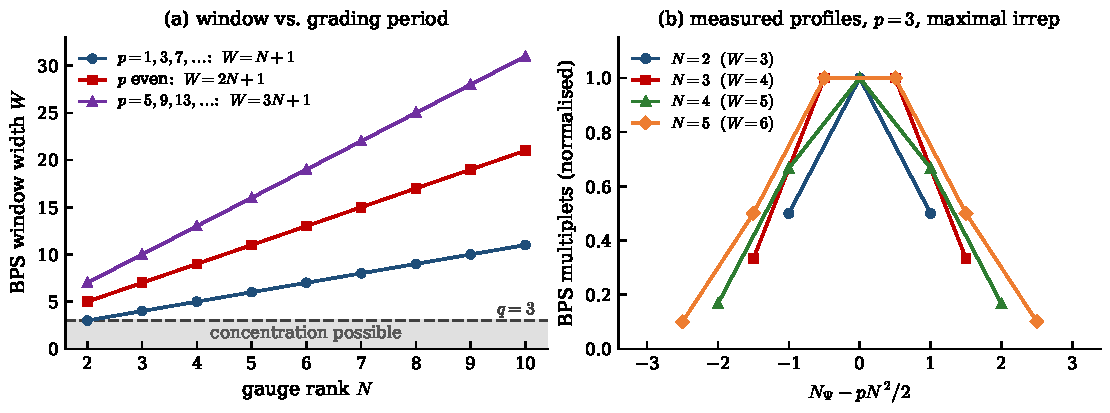
\includegraphics[width=0.96\textwidth]{report_figs/nogo_window.pdf}
\caption{(a) BPS window width against gauge rank. The grading period $q=3$ is fixed (dashed), so concentration is possible only inside the shaded band; every flavour number leaves it at or before $N=3$. (b) Measured BPS multiplet profiles for $p=3$ at the maximal irrep, normalised and centred on half filling: the window visibly widens by one charge per unit of $N$.}
\label{fig:nogo}
\end{figure}

\paragraph{Why concentration fails, and why $N=2$ is misleading.}
The complexes are graded by $c=N_\Psi\bmod3$. A window of $W$ consecutive charges distributes over the three classes with $\lceil W/3\rceil$ charges in the most populated one, so one-degree-per-class requires $W\le3$. At $N=2$, $W=3$ exactly: each class receives exactly one charge and concentration holds --- for purely kinematic reasons, with no input from the dynamics. This is the regime of the $N=2$ evidence cited for the matrix-SYK proposal. From $N=3$ it is arithmetically impossible. At $N=3$ the surplus falls in the $c=0$ class, whose index vanishes, so the extra states are invisible to the index and the non-zero-index classes still saturate; at $N=4$ the surplus falls in $c=1,2$, whose index does \emph{not} vanish, so saturation fails where the index is macroscopic. Across the thirteen highest irreps at $N=4$ we count $3{,}008{,}825{,}568$ BPS states of which $19.0\%$ are invisible to the index.

\paragraph{Robustness.}
The conclusion does not depend on the couplings, the gauge group, or the supercharge degree. (i) \emph{Couplings:} sampling $30$ random cyclic tensors $C$ at $N=3$, $p=3$, $26$ give Chen's profile exactly and $4$ give a \emph{wider} window (width $10$), never a narrower one. (ii) \emph{Casimir:} descending the spectrum at $N=3$ through complete Casimir tiers from $C_2=48$ to $C_2=24$ --- thirteen irreps, up to Fock multiplicity $110\,080$, a factor $215$ above the maximal irrep --- the support is width $4$ in every single case. (iii) \emph{Gauge group:} $su(N)$ removes one Cartan direction and narrows the window by exactly one, so $su(3)$ (rank $2$) concentrates with $h=9,18,9$ while $su(4)$ (rank $3$) does not; the controlling parameter is $\rank G$. (iv) \emph{Degree:} raising $q$ does not help, for the reason given next.

\section{The analytic no-go}\label{sec:analytic}

\paragraph{Factorisation over Cartan slots.}
At the maximal weight $\lambda^*_i=p(N+1-2i)$ every off-diagonal mode is saturated, so the only unoccupied modes are the diagonal ones. A gauge-invariant $Q$ must create a closed index loop, and any loop entering an index cannot leave it --- its outgoing edges are occupied. The surviving loops are therefore \emph{self-loops} at a single index, creating $q$ diagonal modes of distinct flavours. Hence $Q=\sum_{i=1}^{\rank G}Q_i$ with $Q_i$ acting only within slot $i$, and $Q_i$ is wedging with the totally antisymmetric part of $C$. By K\"unneth,
\begin{equation}
Z_{\max}(t)=t^{k_0}\big(z_{\rm slot}(t)\big)^{\rank G},\qquad
z_{\rm slot}(t)=\textstyle\sum_j\dim H^j\big(\Lambda^\bullet\mathbb C^p,\ \omega\wedge\big)\,t^j,\qquad \omega=\mathrm{Alt}(C)\in\Lambda^q\mathbb C^p .
\label{eq:factorise}
\end{equation}
Equation~\eqref{eq:factorise} reproduces all ten measured $u(N)$ cases exactly, across $p=1,2,3,4$, $q=3,5$ and $N=2,\dots,5$. If $z_{\rm slot}$ has support on $w_s$ degrees then the window width is $W=\rank G\,(w_s-1)+1$, which is the law in Table~\ref{tab:widths}.

\paragraph{$w_s\ge2$, and the bound.}
Let $E_c=\sum_{j\equiv c\,(q)}(-1)^j\binom pj$ be the Euler characteristic of the class-$c$ subcomplex of $\Lambda^\bullet\mathbb C^p$; $E_c\ne0$ forces cohomology somewhere in class $c$. Two elementary facts pin this down: $\sum_cE_c=(1-1)^p=0$ for $p\ge1$, so exactly one non-zero $E_c$ is impossible; and $E_c=\tfrac1q\sum_{m=1}^{q-1}\zeta^{-mc}(1-\zeta^m)^p$ with $\zeta=e^{2\pi i/q}$ and $1-\zeta^m\ne0$, so they cannot all vanish. At least two classes therefore carry cohomology, $w_s\ge2$, and
\begin{equation}
W\ \ge\ \rank G+1\qquad\Longrightarrow\qquad \text{concentration}\ \Rightarrow\ \rank G\ \le\ q-1 .
\label{eq:nogo}
\end{equation}
Raising $q$ cannot rescue this. With $\omega\ne0$ (which requires $q\le p$) the minimum of $w_s$ is $q-1$ for $q\ge5$, so $\rank G\le\lfloor(q-1)/(q-2)\rfloor=1$; only $q=3$ attains $w_s=2$, and there $\rank G\le2$. Scanning all $q\le p\le14$, the maximum rank compatible with concentration is \textbf{2}, attained at $q=3$ with $p\equiv3\bmod4$. Scaling $p$ yields infinitely many concentrating models, all at rank $2$.

\paragraph{The free branch.}
One evasion exists and is instructive. If $q>p$ then $\omega\in\Lambda^q\mathbb C^p=0$, the differential vanishes on the sector, $z_{\rm slot}=(1+t)^p$, and for $p=1$ this gives $w_s=2$ with arbitrary $q$, hence unbounded rank. But $\omega=0$ means $Q$ annihilates the sector outright: every state is BPS because nothing acts on it, not because of fortuity. This is the single-matrix, Casimir-solvable situation. It satisfies the counting definition of concentration while being physically its opposite, which shows that the counting criterion alone is not sufficient --- one needs $Q$ to act non-trivially \emph{and} the window to fit inside one period, and \eqref{eq:nogo} says those demands are incompatible beyond rank $2$.

\section{Outlook}

\begin{itemize}
\item \textbf{Close the last gap in the theorem.} The bound $\rank G\le q-1$ is proved; the sharpening to $\rank G\le2$ uses the observed $w_s^{\min}=q-1$ for $q\ge5$, verified at $q=3,5,7,9$ and by an exhaustive scan of $q\le p\le14$. Proving $w_s^{\min}=q-1$ is a self-contained question about $H(\Lambda^\bullet\mathbb C^p,\omega\wedge)$ with no physics in it.
\item \textbf{Beyond the maximal weight.} The factorisation~\eqref{eq:factorise} is derived at the maximal weight and for $u(N)$; it fails for $su(N)$, where Cartan directions straddle slots, which is visible in the anomalous $su(4)$ profile $13,81,81,13$. Empirically the window matches the maximal one throughout the $N=3$ spectrum down to $C_2=24$, but this is not derived.
\item \textbf{The low-Casimir bulk.} The macroscopic-index complexes lie at low Casimir --- at $N=4$ the largest multiplicity is $6.6\times10^9$ at $C_2=20$ --- where weight spaces reach $10^9$ and a genuinely sparse rank routine would be needed. Our coverage spans a factor $215$ in multiplicity at $N=3$ but not the final factor of $\sim5$ to the peak.
\item \textbf{Chaos without concentration.} The three-flavour $H$ is \emph{not} a Casimir function, unlike the single-matrix case, so the model may still be chaotic and have a super-Schwarzian near-BPS spectrum even though its BPS sector is not concentrated. Nothing here bears on that, and it is the natural next question --- Altland--Zirnbauer statistics of the singular values of $Q_k$, now cheap to extract weight by weight.
\item \textbf{What would concentrate.} Equation~\eqref{eq:nogo} says one needs $q$ growing with the rank, and $\omega\ne0$ needs $p\ge q$: an interaction touching $O(N)$ of the $N^2$ matrix entries. Whether such a model is chaotic, or has a sensible large-$N$ limit, is open.
\end{itemize}

\section{Numerical implementation}

All computations are exact integer linear algebra; no floating-point tolerance enters any reported number. Weight bases are enumerated by a pruned recursion over the occupation matrix, validated by $\sum_\lambda\dim W_\lambda(k)=\binom{pN^2}{k}$ for every $k$ at $N=3$ and against the Fock character at $N=4$. Ranks use Gaussian elimination over $\mathbb F_P$ with $P=2^{31}-1$ for small blocks, and for large ones a blocked LU with the trailing update as a BLAS matmul over $P\approx2^{20}$, chosen so that $\text{block}\times(P-1)^2<2^{53}$ keeps every float64 partial sum an exact integer; every rank is confirmed over a second prime. The $\mathbb Z_p$ flavour blocking is performed over $\mathbb F_P$ with $P\equiv1\bmod p$, the eigenbasis built from orbits of the rotation with their fermionic signs, and is validated by requiring the block ranks to sum to the dense rank for every $k$. Kostant multiplicities are computed from the Weyl alternating sum with a pruned partition function and verified against $\sum_\lambda K(\mu,\lambda)=\dim\mu$. Representative costs: the eight highest irreps at $N=3$ in under two minutes at $1.0$\,GB; thirteen irreps at $N=4$ in $30$ minutes at $6.1$\,GB; the $N=5$ maximal weight in $49$ seconds at $0.4$\,GB.

\begin{thebibliography}{9}\small
\bibitem{Chen:2025fortuity} Y.~Chen, \emph{Revisiting fortuity in matrix models}, 2025.
\bibitem{Chang:2024fortuitySYK} C.~Chang, Y.~Chen, W.~Sia, S.~Yang, \emph{Fortuity in SYK models}, 2024.
\bibitem{Chang:2024covering} C.~Chang, Y.~Lin, \emph{Words to describe fortuitous states}, 2024.
\bibitem{Fu:2016SUSYSYK} W.~Fu, D.~Gaiotto, J.~Maldacena, S.~Sachdev, \emph{Supersymmetric SYK models}, Phys.\ Rev.\ D\ \textbf{95} (2017) 026009.
\bibitem{Turiaci:2023N2JT} G.~Turiaci, E.~Witten, \emph{$\mathcal N=2$ JT supergravity and matrix models}, 2023.
\end{thebibliography}

\end{document}
